\chapter{DeepMM: Deep Learning Based Map Matching}

Source: \cite{Feng2020}

未来可阅读方向: \cite{Gong2018, Jagadeesh2014, Yang2018, Lou2009}

\section{论文动机}

HMM算法的缺点:
\label{Problem:PureHMM2}
\begin{itemize}
    \item 只根据当前轨迹进行估计,忽略了历史数据存在的用户移动特征、路网特征
    \item 对于噪声敏感(HMM方法依赖于距离测量),后续方法尽管都考虑到了噪声,但仍旧非常敏感
    \item  HMM是\textbf{基于模型的方法}
\end{itemize}

深度模型快速发展

地图匹配的问题:误差大(在高楼区GPS信号反射);采样率低(能源消耗)

\section{论文贡献}

引入对于真实数据的观察、物理空间的常识去拓展原始数据的量

其他方法忽略了历史数据存在的用户移动特征、路网特征:本文引入seq2seq

其他方法均是基于物理地球距离进行计算:引入嵌入方法,在嵌入空间进行处理)

现实中收集轨迹和事实(ground truth)数据很难:引入数据增强技术


\section{模型设计}

主要框架:通过嵌入方法将位置、路段嵌入高维潜空间(high dimensional latent space),后续在这个空间进行处理;然后通过seq2seq+注意力机制模型从历史数据学习轨迹到路段的映射函数;使用数据增强技术提升效果

\begin{definition}[基于GPS的轨迹]
   $ l = (lon, lat), P_T^l = [l_1, l_2, \cdots]$
\end{definition}

\begin{definition}[基于路段的轨迹]
    $ P^{s}=\left[s_{1}, s_{2}, s_{3}, \ldots\right] $
\end{definition}

\subsection{Statistic-based Data Augmentation}

原始轨迹可以视为是事实的低采样低准确率的粗略版本,可以仿真生成虚拟的GPS轨迹点扩充数据集。

需要两个参数:采样率、空间误差

空间误差假设服从$ f\left(x \mid \mu, \sigma^{2}\right)=\frac{1}{\sqrt{2 \pi \sigma^{2}}} e^{\frac{-(x-\mu)^{2}}{2 \sigma^{2}}} $.

扩充方法:重复多次下采样事实轨迹,添加随机高斯噪声

\begin{remark}
    采样率不固定?误差的模型完全符合高斯分布?(论文数据集支持近似高斯分布)
\end{remark}

\subsection{Generation-based Data Augmentation}

对于已有的轨迹进行数据增强仍旧不足(路网没有全覆盖)

考虑现实中人通常沿着最短路径走,可以生成一些“事实”路径

\begin{itemize}
    \item 通过路网和路径算法生成最短路径: 随机取起点和终点,通过Graphhopper routing engine:基于Dijkstra算法规划最短路径
    \item 修正最短路径使得它更真实:
    \item 通过上一节的方法加入噪声
\end{itemize}

\subsubsection{修正最短路径}

根据路径长度$d$随机选择$N_W$个停留点、定位点、路径点(waypoint)$W$

\begin{equation} N_{W}=d / \alpha * p \end{equation}

对于这些点加入与长度成正比的噪声。

\subsection{Attentional seq2seq Model}

\begin{figure}[htbp]
    \caption{Attentional sequence to sequence model. The encoder uses a
    BiLSTM to encode the input trajectory as a vector. The decoder uses a
    LSTM to decode the target sequence from the vector.}
    \centering
    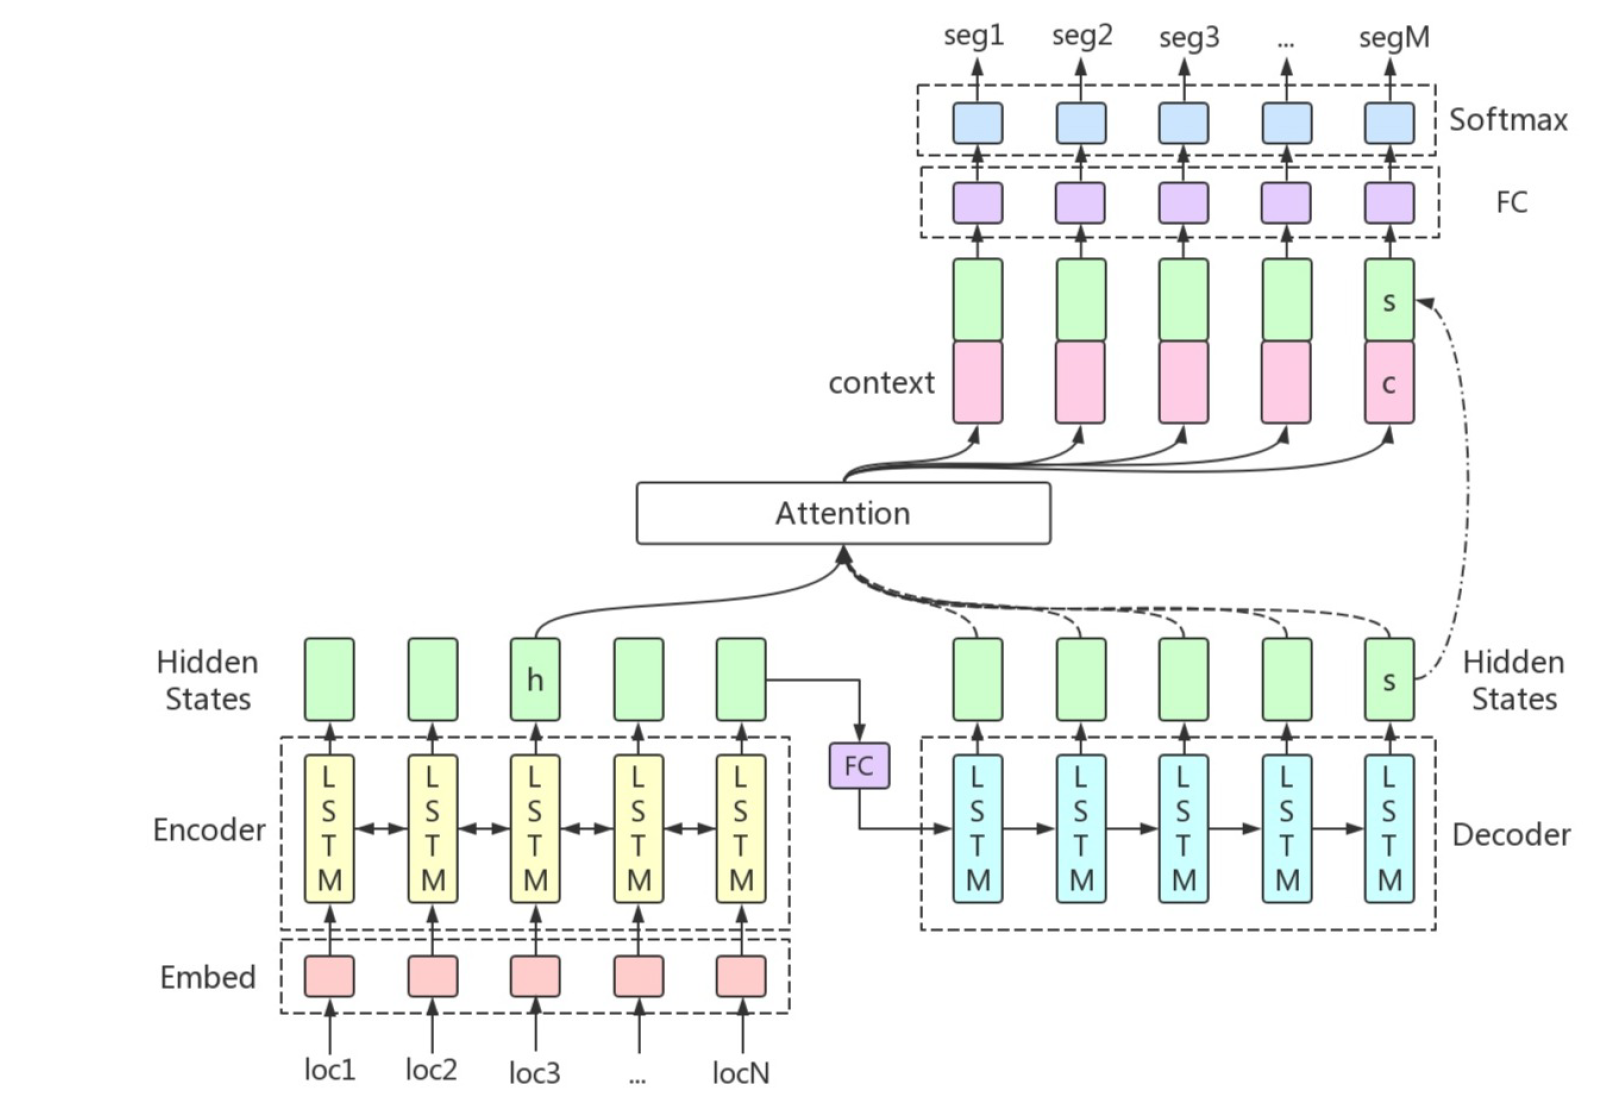
\includegraphics[width=\textwidth]{HMM-DeepHMM-architecture.png}
\end{figure}

encoder输入:位置嵌入模块(将输入的轨迹上下文信息转化为潜空间的密集向量)(双向多层LSTM)

decoder输出:LSTM(从向量中转译回一个序列)

注意力机制:捕捉长程、复杂的依赖

\subsubsection{Location Embedding}

HMM只对相邻状态之间的转移进行了建模,忽略了用户的偏好 \cite{Jagadeesh2017} 和道路信息 \cite{Hu2017a}.

借鉴NLP tokenization的方法,将地图划分为100*100的网格,每个网格编号一个ID.对于每个ID转换为one-hot向量,对于轨迹生成一串one-hot序列输入seq2seq的模型中

\begin{remark}
    轨迹不定长?
\end{remark}

\subsubsection{Sequential Encoder}

RNN是一个处理序列数据的模型,但是它太简单。使用LSTM作为基本单元。

堆叠双向LSTM抽取输入的轨迹信息。

\subsubsection{Attentional Decoder}

输入decoder之前的FC是用于调整维度。解码器需要是单向的LSTM. decoder的中间输出会被FC和Softmax进行处理。decoder一次生成一个点直到stop mark.

seq2seq的输入输出不需要是同样长度(灵活—)

由于轨迹很长,而seq2seq每次只传送一个向量到decoder,可能损失长程信息。因此引入注意力机制高效地重新访问中间隐状态。

decoder的隐状态$s_i$和每一个encoder的隐状态$h_i$的相关性:

\begin{equation} \alpha_{i, j}=\frac{\exp \left(e_{i, j}\right)}{\sum_{k=1} \exp \left(e_{i, k}\right)} \end{equation}

where $ e_{i, j}=s_{i} * h_{j} $

encoder的隐状态$h$ 经过加权形成一个上下文向量$c_i$

\begin{equation} c_{i}=\sum_{j=1} \alpha_{i, j} h_{j} \end{equation}

\subsection{Trajectory Calibration and Topology Refinement}

OSM中的默认路段\textbf{不是基于道路的交叉口},这意味着用户可能\textbf{不会通过整个路段并在交叉口掉头}.(OSM数据的交叉点还是粒度太高,车辆可能从路中间转向)

此外,虽然模型期望直接从真实数据中学习拓扑连续性,但在\textbf{训练过程中无法保证拓扑连续性}.因此需要轨迹标定和精化方案,以获得合理的结果和更好的匹配性能。

对匹配出的路段在中间进行剪枝

\section{实验}

对比方法:

\begin{definition}[Fast MM(FMM)]
    \cite{Yang2018} FMM integrates Hidden
Markov Model with two acceleration mechanisms: 1)
pre-computing upper bounded origin-destination table to
store all pairs of shortest paths; 2) replacing the repeated
routing queries with fast hash table search.
\end{definition}

\begin{definition}[ST Matching]
    \cite{Lou2009} It is a global map-matching algorithm
    for low-sampling-rate GPS trajectories. With considering
    the spatial and topological structures of the road network
    and temporal features of trajectories, it constructs a candidate
    graph to find the best matching path sequence
\end{definition}

测量指标:


 \begin{equation}\text{accuracy} =\frac{\operatorname{len}\left(P^{s m} \cap P^{s g}\right)}{\max \left\{\operatorname{len}\left(P^{s m}\right), \operatorname{len}\left(P^{s g}\right)\right\}} \end{equation}

 \textbf{Spatial skewing} indicates
the average distance of the matched locations to the ground
truth locations.
  \begin{equation}\text{spatial skewing} =\frac{\sum_{i} \min _{j} \operatorname{dist}\left(P_{i}^{l g} P_{j}^{l m}\right)}{\operatorname{len}\left(P^{l g}\right)} \end{equation}

基于扩充数据训练的深度学习模型比传统方法具有更好的学习人类运动模式的能力,并且在匹配过程中通过注意力机制更好地考虑了全局信息。